\documentclass[a4paper, 11pt, twocolumn]{article}
\usepackage[utf8]{inputenc}
\usepackage{graphicx}
\usepackage[noend]{algorithm2e}
\usepackage{float}
\usepackage{amsmath}
\usepackage{amssymb}
\usepackage{epsfig,floatflt}
\usepackage{physics}
\usepackage[english]{babel}
\usepackage{booktabs}
\usepackage[round]{natbib}
%\usepackage{cite}
\usepackage[format=plain,
font=it]{caption}
\usepackage{url}
\usepackage{hyperref}
\usepackage{color}
\definecolor{darkred}{rgb}{0.5,0,0}
\definecolor{darkgreen}{rgb}{0,0.5,0}
\definecolor{darkblue}{rgb}{0,0,0.5}


\hypersetup{ colorlinks,
	linkcolor=darkblue,
	filecolor=darkgreen,
	urlcolor=darkred,
	citecolor=darkblue }

\graphicspath{{../figures/}}
\DeclareGraphicsExtensions{.pdf}

\begin{document}

\title{Numerical exploration of Rossby waves}

\author{Jan-Adrian Kallmyr}

\twocolumn[
  \begin{@twocolumnfalse}
    \maketitle
%    \begin{abstract}

\end{abstract}

  \end{@twocolumnfalse}
]

\section{Introduction}
\label{sec:introduction}



\section{Theory}
\label{sec:theory}

The linearized shallow water equations are as follows:
	\begin{align}
		&\partial_t u - f_0 v = -g \partial_x h \label{eq:dudt} \\
		&\partial_t v + f_0 u = -g \partial_y h \label{eq:dvdt} \\
		&\partial_t h + D_0 \qty(\partial_x u + \partial_y v) = 0, \label{eq:dhdt}
	\end{align}
where $\partial_{q_i}$ denotes partial differentiation or ordinary differentiation given the context. $u$ and $v$ are the zonal and meridional velocities, respectively, while $h$ is the sea-surface height. The planetary vorticity is $f_0$, while $g$ is the gravitational acceleration, and $D_0$ is the depth of the system. 

In this report, we will study the case of a stepwise sea surface height perturbation of $\pm h_0$
	\begin{equation}
		h_i = h_0
			\begin{cases}
			h_0, & x > 0 \\
			-h_0, & x < 0
			\end{cases},
	\label{eq:initial_h}
	\end{equation}
which can be solved analytically.

\subsection{Dynamics}
The resulting sea surface height after geostrophic adjustment is
	\begin{equation}
		h_f = h_0
			\begin{cases}
				-1 + \exp(-x / R), & x > 0\\
				1 - \exp(x / R), & x < 0
			\end{cases},
	\label{eq:analytical_h}
	\end{equation}
where $R \equiv \sqrt{gD_0} / f_0$ is the Rossby radius of deformation, i.e. the length scale where rotational effects are important. In geostrophic balance, the meridional velocity is just $v = -\partial_x h$, giving
	\begin{equation}
		v = -\frac{g h_0}{f_0R} \exp(-\abs{x} / R)
	\label{analytical_v}
	\end{equation}
for the final state.

\subsection{Energetics}
The total energy of a system with density $\rho$ can be decomposed into potential and kinetic components
	\begin{align}
		V &= \frac{1}{2}\rho g \qty(h^2 - D^2_0) \\
		K &= \frac{1}{2}\rho D_0 \qty(u^2 + v^2),
	\end{align}
and the available potential energy is obtained by subtracting the constant term.
For an initial height perturbation eq. \ref{eq:initial_h} the resulting change in available potential and kinetic energy is
	\begin{align}
		\Delta V &= - \frac{3}{2} \rho g h^2_0 R \label{eq:change_potential} \\
		\Delta K &= \frac{1}{2} \rho g h^2_0 R \label{eq:change_kinetic}.
	\end{align}
Initially, the potential energy constitutes the total energy, and so from eqs. \ref{eq:change_potential} and \ref{eq:change_kinetic} the final kinetic energy should be a 1/3 of the total energy. Likewise, the potential energy should be a 2/3 of the total energy.

\section{Method}
\label{sec:method}
We will follow the same dicretization scheme and method as done in a previous paper \citep{lab1}, with some further implementations of reduced gravity and the beta plane.

The initial condition is a gaussian centered at the equator
	\begin{equation}
		h_i = h_0\exp\qty[-((x - 0.5*L_x)/L_w)^2 - (y/L_w)^2],
	\end{equation}
where $L_i$ denotes the domain size and $L_w$ is a scaling factor.

For studying the southern border, we will assume periodic boundary conditions in the zonal direction and a open northern border. We will look at two different cases, that of the Atlantic ocean and the Baltic sea with basin parameters shown in Table \ref{tab:southernborder}.
	\begin{table}[htbp]
		\begin{tabular}{lll}
			\textbf{Region} & \textbf{L}  & \textbf{D}$'_0$  \\
			Atlantic ocean & $10^7\, \text{m}$  & $1000\, \text{m}$  \\
			Baltic sea & $10^6\, \text{m}$ & $30\, \text{m}$ 
		\end{tabular}
		\caption{Basin parameters for the Atlantic ocean and Baltic sea. $L$ denotes the domain size, while $D'_0$ is the thermocline depth.}
		\label{tab:southernborder}
	\end{table}

When looking at the equatorial wave, we use solid boundaries in all directions with domain size $L = 2 \cdot 10^7\, \text{m}$ and thermocline depth $D'_0 = 1000\, \text{m}$.

Global parameters for the simulations are presented in Table \ref{tab:parameters}
	\begin{table}[htbp]
		\begin{tabular}{ll}
			\textbf{Parameter} & \textbf{Value} \\
			$ g' $ & $ 0.04 \, \text{m}\text{s}^{-2} $ \\
			$ f_0 $ & $ 10^{-4} \, \text{s}^{-1}$ \\
			$ \beta $ & $ 2.287 \cdot 10^{-11} \, \text{ (sm) }^{-1}  $
		\end{tabular}
		\caption{Model parameters.}
		\label{tab:parameters}
	\end{table}

\section{Results}
\label{sec:results}

\begin{figure}[htbp]
	\centering
	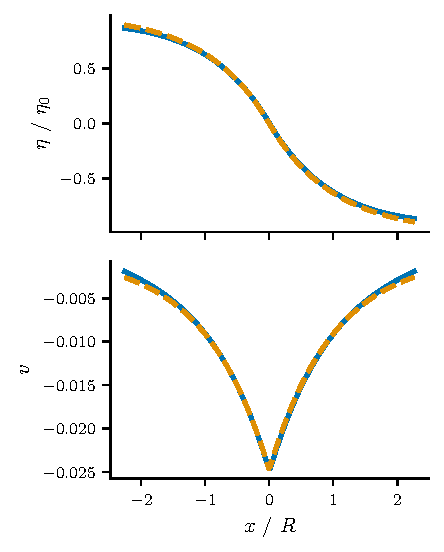
\includegraphics{dynamics_comparison}
	\caption{Upper: relative sea surface height. Lower: meridional velocity. Solid line shows numerical result, while dashed line shows analytical results.}
	\label{fig:dynamics}
\end{figure}

\begin{figure}[htbp]
	\centering
	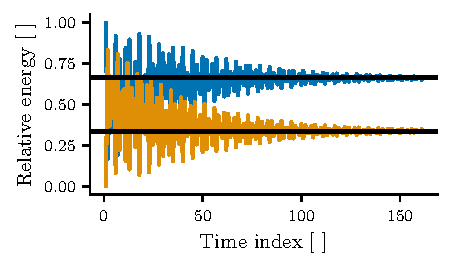
\includegraphics{energetics}
	\caption{Relative energies where blue line shows potential energy and orange line shows kinetic energy.}
	\label{fig:energetics}
\end{figure}

\section{Discussion}
\label{sec:conclusion}

While Figure \ref{fig:dynamics} shows that there is high agreement between the numerical and analytical solutions, this result is dependent on the size of the sponge used for the periodic boundary conditions. In essence, some tuning is necessary to achieve this result, and should be taken into account. Another question may be why the final state is not that of a flat ocean surface, and this would indeed be the cause in a non-rotating system where no force can balance the pressure gradients. In a rotating system, however, this is achieved by the coriolis force.

Figures \ref{fig:energetics_d} and \ref{fig:energetics_f} illustrates that the planetary vorticity and depth have reverse effects on the result, which is not surprising due to their competing dependency in the Rossby radius of deformation. Increasing the depth or reducing the planetary vorticity will increase $R$, which allows for greater potential energy retention due to a larger area where the coriolis force can balance the pressure gradients.

\subsection{Conclusion}
In this report we have studied the dynamics and energetics of geostrophic adjustment by solving the shallow water equations numerically and analytically for a step-wise sea surface height perturbation. We found general good agreement between numerical and analytical solutions. Exploring the effect of changing the Rossby radius, we found that a larger Rossby radius tends to cause a greater fraction of the total energy to be potential energy. This was due to a overall larger contribution from rotational effects balancing pressure gradients.


\bibliographystyle{plainnat}

\bibliography{ourbib}



\end{document}
